%%%%%%%%%%%%%%%%%%%%%%%%%%%%%%%%%%%%%%%%%%%%%%%%%%%%%%%%%%%%%%%%%%%%%%%%%%%%%%%
%
% Filename: template.tex
% Author:   David Oniani
% Modified: January 03, 2021
%  _         _____   __  __
% | |    __ |_   _|__\ \/ /
% | |   / _` || |/ _ \\  /
% | |__| (_| || |  __//  \
% |_____\__,_||_|\___/_/\_\
%
%%%%%%%%%%%%%%%%%%%%%%%%%%%%%%%%%%%%%%%%%%%%%%%%%%%%%%%%%%%%%%%%%%%%%%%%%%%%%%%

%%%%%%%%%%%%%%%%%%%%%%%%%%%%%%%%%%%%%%%%%%%%%%%%%%%%%%%%%%%%%%%%%%%%%%%%%%%%%%%
% Document Definition
%%%%%%%%%%%%%%%%%%%%%%%%%%%%%%%%%%%%%%%%%%%%%%%%%%%%%%%%%%%%%%%%%%%%%%%%%%%%%%%

\documentclass[11pt]{article}

%%%%%%%%%%%%%%%%%%%%%%%%%%%%%%%%%%%%%%%%%%%%%%%%%%%%%%%%%%%%%%%%%%%%%%%%%%%%%%%
% Packages and Related Settings
%%%%%%%%%%%%%%%%%%%%%%%%%%%%%%%%%%%%%%%%%%%%%%%%%%%%%%%%%%%%%%%%%%%%%%%%%%%%%%%

% Global, document-wide settings
\usepackage[margin=1in]{geometry}
\usepackage[utf8]{inputenc}
\usepackage[english]{babel}

% Other packages
\usepackage{booktabs}
\usepackage{hyperref}
\usepackage{mathtools}
\usepackage{amsthm}
\usepackage{amssymb}
\usepackage{tikz}
\usepackage[cache=false]{minted}

%%%%%%%%%%%%%%%%%%%%%%%%%%%%%%%%%%%%%%%%%%%%%%%%%%%%%%%%%%%%%%%%%%%%%%%%%%%%%%%
% Command Definitions and Redefinitions
%%%%%%%%%%%%%%%%%%%%%%%%%%%%%%%%%%%%%%%%%%%%%%%%%%%%%%%%%%%%%%%%%%%%%%%%%%%%%%%

% Nice-looking underline
\newcommand\und[1]{\underline{\smash{#1}}}

% Line spacing is 1.5
\renewcommand{\baselinestretch}{1.5}

% Absolute value
\DeclarePairedDelimiter\abs{\lvert}{\rvert}%

% Absolute value big
\DeclarePairedDelimiter\absb{\Big\lvert}{\Big\rvert}%

% Ceiling
\DeclarePairedDelimiter{\ceil}{\lceil}{\rceil}

% Ceiling big
\DeclarePairedDelimiter{\ceilb}{\Big\lceil}{\Big\rceil}

% Floor
\DeclarePairedDelimiter\floor{\lfloor}{\rfloor}

% % Naturals, Reals, Integers, and Rationals, 
\newcommand{\nats}{\mathbb{N}}
\newcommand{\reals}{\mathbb{R}}
\newcommand{\preals}{\mathbb{R^+}}
\newcommand{\nreals}{\mathbb{R^-}}
\newcommand{\ints}{\mathbb{Z}}
\newcommand{\pints}{\mathbb{Z^+}}
\newcommand{\nints}{\mathbb{Z^-}}
\newcommand{\rats}{\mathbb{Q}}
\newcommand{\prats}{\mathbb{Q^+}}
\newcommand{\nrats}{\mathbb{Q^-}}
\newcommand{\irrats}{\mathbb{I}}
\newcommand{\pirrats}{\mathbb{I^+}}
\newcommand{\nirrats}{\mathbb{I^-}}

%%%%%%%%%%%%%%%%%%%%%%%%%%%%%%%%%%%%%%%%%%%%%%%%%%%%%%%%%%%%%%%%%%%%%%%%%%%%%%%
% Miscellaneous
%%%%%%%%%%%%%%%%%%%%%%%%%%%%%%%%%%%%%%%%%%%%%%%%%%%%%%%%%%%%%%%%%%%%%%%%%%%%%%%

% Setting stuff
\setlength{\parindent}{0pt}  % Remove indentations from paragraphs

% PDF information and nice-looking urls
\hypersetup{%
  pdfauthor={David Oniani},
  pdftitle={Real Analysis},
  pdfsubject={Mathematics, Real Analysis, Real Numbers},
  pdfkeywords={Mathematics, Real Analysis, Real Numbers},
  pdflang={English},
  colorlinks=true,
  linkcolor={black!50!blue},
  citecolor={black!50!blue},
  urlcolor={black!50!blue}
}

%%%%%%%%%%%%%%%%%%%%%%%%%%%%%%%%%%%%%%%%%%%%%%%%%%%%%%%%%%%%%%%%%%%%%%%%%%%%%%%
% Author(s), Title, and Date
%%%%%%%%%%%%%%%%%%%%%%%%%%%%%%%%%%%%%%%%%%%%%%%%%%%%%%%%%%%%%%%%%%%%%%%%%%%%%%%

% Author(s)
\author{David Oniani\\
        Luther College\\
        \href{mailto:oniada01@luther.edu}{oniada01@luther.edu}}

% Title
\title{\rule{\paperwidth - 150pt}{1pt}\textbf{\\\textit{Real Analysis
Exams}\\}\rule {\paperwidth - 150pt}{1pt}\\\textbf{Exam
\textnumero2}\\{\normalsize Instructor: Dr. Eric Westlund}}

% Date
\date{\today}

%%%%%%%%%%%%%%%%%%%%%%%%%%%%%%%%%%%%%%%%%%%%%%%%%%%%%%%%%%%%%%%%%%%%%%%%%%%%%%%
% Beginning of the Document
%%%%%%%%%%%%%%%%%%%%%%%%%%%%%%%%%%%%%%%%%%%%%%%%%%%%%%%%%%%%%%%%%%%%%%%%%%%%%%%

\begin{document}
\maketitle

%%%%%%%%%%%%%%%%%%%%%%%%%%%%%%%%%%%%%%%%%%%%%%%%%%%%%%%%%%%%%%%%%%%%%%%%%%%%%%%

\begin{itemize}
    \item[1.]
        \begin{itemize}
            \item[(a)]
                Let $S_n = (a - \frac{1}{n}, b + \frac{1}{n})$. Then $S_n$ is
                open. Now, it is easy to see that $S = \cap_{n = 1}^{\infty}
                S_n$ is $G_\delta$ set. Furthermore, $[a, b] \subseteq S$ as
                $\forall n, [a, b] \subseteq S_n$. Now, suppose, for the sake
                of contradiction, that $x \in S$ and $x \notin [a, b]$. We have
                two cases:
                \begin{itemize}
                    \item[(i)]
                        $x < a \implies \exists n$ s.t. $a - x > \frac{1}{n}$
                        and thus, $x < a - \frac{1}{n}$. It follows that $x
                        \notin S_n$ and $x \notin S$. Hence, we face a
                        contradiction and $x \geq a$.

                    \item[(ii)]
                        $x > b \implies \exists n$ s.t. $x - b > \frac{1}{n}$
                        and thus, $x > b + \frac{1}{n}$. It follows that $x
                        \notin S_n$ and $x \notin S$. Hence, we face a
                        contradiction and $x \leq b$.
                \end{itemize}
                Finally, from these two cases, we got that $x \geq a$ and $x
                \leq b$ and thus $x \in [a, b]$. Therefore, $[a, b]$ is
                $G_\delta$ set.

            \item[(b)]
                Let $S_n = (a, b + \frac{1}{n})$. Then, by the argument
                presented in $(a)$ part of the exercise, $S = \cap_{n =
                1}^{\infty} S_n = (a, b]$ and thus $(a, b]$ is $G_\delta$.
                \\
                \\
                Now, suppose, for the sake of contradiction, that $U_n = [a +
                \frac{1}{n}, b], x \in U_n$, and $ x \notin (a, b]$. Let us now
                consider these two cases:
                \begin{itemize}
                    \item[(i)]
                        $x \leq a \implies x < a + \frac{1}{n} \implies x
                        \notin U_n$ and we face a contradiction.

                    \item[(ii)]
                        $x > b \implies x \notin U_n$ and we face a
                        contradiction.
                \end{itemize}
                Thus $x > a$ and $x \leq b$ which implies that $x \in (a, b]$
                and therefore, $(a, b]$ is $F_\sigma$. Hence, we have shown
                that any arbitrary half-open interval $(a, b]$ is both
                $G_\delta$ and $F_\sigma$.

            \item[(c)]
                To prove that $\rats$ is $F_\sigma$, we need to find a
                countable collection of closed subsets of $\rats$ whose union
                is $\rats$. Now, since $\rats$, there exists a bijective
                function $f : \nats \to \rats$. Then, $\forall n \in \nats$,
                set $S_n = \{f(n)\}$ is closed. We have $\rats =
                \displaystyle\bigcup_{n = 1}^{\infty} \{S_n\}$ is a union of
                closed sets. Thus, by definition, $\rats$ is $F_\sigma$ set.

            \item[(d)]
                Notice that $\reals - \rats$ is the set of irrational numbers
                which is the complement of the rational numbers in $\reals$.
                Hence, $\irrats = \reals - \rats = \rats^c$. From $(c)$ we know
                that $\rats$ can be represented as a countable union of closed
                sets. Then, per \textbf{De Morgan's Law}, we get that $\irrats$
                is the countable intersection of open sets (complement of a
                closed set is an open set). Hence, by definition, we get that
                $\reals - \rats$ is $G_\delta$.

            \item[(e)]
                Since this is a if and only if question, let us first prove
                the statement directly and then prove its converse.
                \begin{itemize}
                    \item[(i)]
                        Let us first show that a set is a $G_\delta$ set if
                        its complement is an $F_\sigma$ set.
                        \\
                        \\
                        Suppose that we have a set $S$ which is a $G_\delta$
                        set. Then, by definition, $S = \displaystyle\bigcap_{n
                        = 1}^{\infty}S_n$ where every $S_n$ is an open set.
                        Then, by \textbf{De Morgan's Law}, it follows that $S^c
                        = \displaystyle\bigcup_{n = 1}^{\infty}S_n^c$ (with
                        $S_n^c$ being closed as the complement of an open set
                        is a closed set) and by definition, $S^c$ is a
                        $F_\sigma$ set.\\
                        $\qed$

                    \item[(ii)]
                        Let us now prove the converse, that if a set is a
                        complement of a $F_\sigma$ set, then it is a $G_\delta$
                        set.
                        \\
                        \\
                        Suppose that we have a set $S$ which is a $F_\sigma$
                        set. Then, by definition, $S = \displaystyle\bigcup_{n
                        = 1}^{\infty}S_n$ where every $S_n$ is a closed set.
                        Then, by \textbf{De Morgan's Law}, it follows that $S^c
                        = \displaystyle\bigcap_{n = 1}^{\infty}S_n^c$ (with
                        $S_n^c$ being open as the complement of a closed set is
                        an open set) and by definition, $S^c$ is a $F_\sigma$
                        set.\\
                        $\qed$
                \end{itemize}
                Finally, we have proven that a set is a $G_\delta$ set if and
                only if its complement is an $F_\sigma$ set.\\
                $\qed$
        \end{itemize}

    \item[2.]
        Let us first prove that
        $\dfrac{1}{2}\mathbb{C} + \dfrac{1}{2}\mathbb{C} = [0, 1]$.
        Recall that the Cantor set $\mathbb{C}$ is the set of all numbers in
        $[0, 1]$ that in the \textbf{ternary system} can be represented as the
        sequence of $0$s and $2$s only. Then $\dfrac{1}{2}\mathbb{C}$ must only
        contain $0$s and $1$s. Now, let $r \in [0, 1]$. If we show that $\exists
        x, y \in \dfrac{1}{2}\mathbb{C}$ s.t $x + y \in [0, 1]$, then we have
        effectively shown that
        $\dfrac{1}{2}\mathbb{C} + \dfrac{1}{2}\mathbb{C} = [0, 1]$. Let us
        construct $x$ and $y$ in the following manner:
        \begin{itemize}
            \item[*]
                Let $x$ have $0$s in the same places where it is in $r$ and let
                $x$ have $1$s when the corresponding digit in $r$ is either $1$
                or $2$.

            \item[*]
                Let $y$ have $0$s in the same places where $r$ has $0s$ or
                $1$s. Let $y$ have $1$s when the corresponding digit in $r$ is
                $2$.
        \end{itemize}
        Hence, we split all $2$s in $r$ in a way that half goes to $x$ and half
        goes to $y$, and all $1$s of $r$ were given to $x$. Thus, $x + y = r$.
        For instance, if $r = 0.120120\dots$, then $x = 0.110110\dots$ and $y =
        0.010010\dots$. It follows that $x + y = 0.120120\dots = r$. Now, since
        we have already shown that
        $\dfrac{1}{2}\mathbb{C} + \dfrac{1}{2}\mathbb{C} = [0, 1]$, we can just
        multiply both sides of the equation by $2$ and we get
        $\mathbb{C} + \mathbb{C} = [0, 2]$.\\
        $\qed$

    \item[3.]
        \begin{itemize}
            \item[(a)]
                $F_2 = \Big[0, \dfrac{4}{25}\Big] \cup \Big[\dfrac{6}{25},
                \dfrac{2}{5}\Big] \cup \Big[\dfrac{3}{5}, \dfrac{19}{25}\Big]
                \cup \Big[\dfrac{21}{25}, 1\Big]$.
                \\
                \\
                Below find the sketch (blue segments are included and red
                segments are not included).
                \\
                \begin{figure}[H]
                    \centering
                    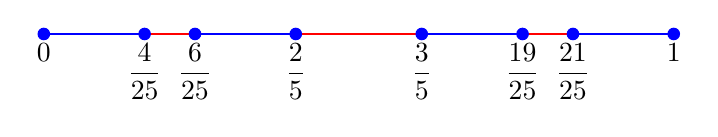
\begin{tikzpicture}[scale=0.8]
                        % X-axis
                        \draw[red] (0,0) -- (10,0);
                        \draw[red] (0,0) -- (10,0);

                        % [0, 4/25]
                        \draw[black] (0, 0) node[below] {0};
                        \fill[blue] (0, 0) circle (0.1);

                        \draw[black] (1.6, 0) node[below] {$\dfrac{4}{25}$};
                        \fill[blue] (1.6, 0) circle (0.1);

                        \draw[blue] (0, 0) -- (1.6, 0);
                        \draw[blue] (0, 0) -- (1.6, 0);

                        % [6/25, 2/5]
                        \draw[black] (2.4, 0) node[below] {$\dfrac{6}{25}$};
                        \fill[blue] (2.4, 0) circle (0.1);

                        \draw[black] (4, 0) node[below] {$\dfrac{2}{5}$};
                        \fill[blue] (4, 0) circle (0.1);

                        \draw[blue] (2.4, 0) -- (4, 0);
                        \draw[blue] (2.4, 0) -- (4, 0);

                        % [3/5, 19/25]
                        \draw[black] (6, 0) node[below] {$\dfrac{3}{5}$};
                        \fill[blue] (6, 0) circle (0.1);

                        \draw[black] (7.6, 0) node[below] {$\dfrac{19}{25}$};
                        \fill[blue] (7.6, 0) circle (0.1);

                        \draw[blue] (6, 0) -- (7.6, 0);
                        \draw[blue] (6, 0) -- (7.6, 0);

                        % [21/5, 1]
                        \draw[black] (8.4, 0) node[below] {$\dfrac{21}{25}$};
                        \fill[blue] (8.4, 0) circle (0.1);

                        \draw[black] (10, 0) node[below] {$1$};
                        \fill[blue] (10, 0) circle (0.1);

                        \draw[blue] (8.4, 0) -- (10, 0);
                        \draw[blue] (8.4, 0) -- (10, 0);
                    \end{tikzpicture}
                    \caption{Sketch of $F_2$.}
                \end{figure}

            \item[(b)]
                Notice that by definition, $F$ is bounded by $[0, 1]$. Recall
                that arbitrary intersection of closed sets is closed (we have
                proved this in the past as a part of an exercise). Now, every
                $F_n$ is closed and since $F$ is an intersection of such sets,
                it follows that $F$ closed. Finally, $F$ is both closed and
                bounded and by \textbf{Theorem 3.3.8 (Heine–Borel Theorem)},
                $F$ is compact.\\
                $\qed$
                
            \item[(c)]
                Notice that in order to construct $F$, we first remove 1
                interval of length $\dfrac{1}{5}$. Then we remove 4
                intervals of length $\dfrac{1}{25}$, then 16 intervals of
                the length $\dfrac{1}{125}$, etc. Thus, the removed intervals
                form the infinite geometric series of the following form:
                \begin{equation*}
                    \dfrac{1}{5} \times \Big(\dfrac{4}{5}\Big)^0, \dfrac{4}{5}
                    \times \Big(\dfrac{4}{5}\Big)^1, \dfrac{1}{5} \times
                    \Big(\dfrac{4}{5}\Big)^2 \dots
                \end{equation*}
                Recall that the sum of such series is calculated by the formula
                $S = \dfrac{s_1}{1 - r}$ where $s_1$ is the first element of
                the sequence and $r$ is the ratio/quotient (next element over
                the previous one). Then, we have $S = \dfrac{\frac{1}{5}}{1 -
                \frac{4}{5}} = \dfrac{\frac{1}{5}}{\frac{1}{5}} = 1$. Now,
                notice that we had the length of $1$ initially as the length of
                $[0, 1]$ is 1. We subtracted $S = 1$ from 1 and get $1 - 1 =
                0$. Thus, the length of $F$ is $0$.

            \item[(d)]
                Suppose, for the sake of contradiction, that $S = \{s_1, s_2,
                \dots\}$ is countable. We now need to find some point $x \in F$
                s.t. $x \notin S$. Notice that $F \subseteq [0, \frac{2}{5}],
                [\frac{3}{5}, 1]$ with $s_1 \notin [0, \frac{2}{5}] \cup [0,
                \frac{2}{5}]$ (i.e., $s_1$ is not in either of the two
                intervals). Let us denote $[0, \frac{2}{5}]$ as $I_1$. Then
                $s_1 \notin I_1$. Similarly, after removing the middle fifth of
                $I_1$, $s_1$ will not be in neither of the resulting two
                intervals and $s_2 \notin I_2$ (where $I_2$ is one of the
                intervals [does not matter which one] obtained after removing
                the middle half of $I_1$, so $I_2 \subset I_1$). If we continue
                in this fashion, after $m$ steps, we get $I_m \subset I_{m - 1}
                \dots \subset I_2 \subset I_1$ with $s_m \notin I_m$. Finally,
                we have found a point $x \in \displaystyle\bigcap_{n =
                1}^{\infty}I_n$ s.t. $x \in F$ but $\forall n, x \neq s_n$.
                Hence, we face a contradiction and $F$ is uncountable.\\
                $\qed$

            \item[(e)]
                Notice that $F_1$ has $2$ intervals of the length
                $\frac{2}{5}$. $F_2$, on the other hand, has $2^2$ intervals of
                the size $\frac{2^2}{5^2}$. $F_3$ consists of $2^3$ intervals
                of the size $\frac{2^3}{5^3}$ and so forth. Hence, in general,
                $F_n$ consists of $2^n$ intervals of the size $\frac{2^n}{5^n}
                = \Big(\frac{2}{5}\Big)^n$. Hence, magnifying $F$ by the factor
                of $\frac{5}{2}$ will give us $2$ additional copies of $F$.
                The equation will be $2 = \Big(\frac{5}{2}\Big)^n$ (for
                instance, $[0 ,1] \times 2.5 = [0, 2.5]$ and after taking the
                middle-fifth, we get two copies $[0, 1]$ and $[1.5, 2.5]$) and
                thus, the dimension of $F$ is
                \begin{equation*}
                    \boxed{\dim{F} = \dfrac{\log{2}}{\log{\frac{5}{2}}} =
                    \dfrac{\log{2}}{\log{5} - \log{2}}}
                \end{equation*}
        \end{itemize}
    
    \newpage

    \item[4.]
        \begin{itemize}
            \item[(a)]
                According to \textbf{Definition 4.2.1 (Functional Limit)},
                we have to show that $\forall \epsilon > 0, \exists \delta > 0$
                s.t. $0 < \abs{x - 3} < \delta \implies \abs{x^2 - 5x + 4 -
                (-2)} < \epsilon$. Let $\epsilon > 0$ be given. Let
                $\delta = -0.5 + \sqrt{0.25 + \frac{\epsilon}{2}}$
                ($\delta > 0$ since $\sqrt{0.25 + \frac{\epsilon}{2}} > 0.5$).
                Then suppose that $\abs{x - 3} = \abs{x - 3} < -0.5 +
                \sqrt{0.25 + \frac{\epsilon}{2}}$
                Notice that:
                \begin{align*}
                    \abs{x^2 - 5x + 4 - (-2)} &= \absb{x^2 - 5x + 6}\\
                                              &= \absb{(x - 2)(x - 3)}\\
                                              &= \absb{-0.5 + \sqrt{0.25 + \frac{\epsilon}{2}} + 1} \times \absb{-0.5 + \sqrt{0.25 + \frac{\epsilon}{2}}}\\
                                              &< \absb{\sqrt{0.25 + \frac{\epsilon}{2}} + 0.5} \times \absb{\sqrt{0.25 + \frac{\epsilon}{2}} - 0.5}\\
                                              &= \absb{0.25 + \frac{\epsilon}{2} - 0.25}\\
                                              &= \absb{\frac{\epsilon}{2}} = \frac{\epsilon}{2} < \epsilon
                \end{align*}
                Hence, we showed that $\forall \epsilon > 0, \exists \delta =
                -0.5 + \sqrt{0.25 + \frac{\epsilon}{2}}$ s.t.
                $0 < \abs{x - 3} < \delta \implies \abs{x^2 - 5x + 4 - (-2)} <
                \epsilon$.\\
                $\qed$

            \item[(b)]
                Per \textbf{Exercise 4.2.9 (b)} that I have completed as a part
                of the assignment, we can say $\lim_{x \to \infty} f(x) = L$ if
                $\forall \epsilon > 0, \exists M > 0$ s.t. if $x > M$ we have
                $\abs{f(x) - L} < \epsilon$. Let us now show that $\lim_{x \to
                \infty} \dfrac{2x}{x + 4} = 2$. Let $\epsilon > 0$ be given and
                let $M = \dfrac{8}{\epsilon}$. Then if $x > M$, we have
                $x > \dfrac{8}{\epsilon}$. We have
                $\dfrac{2x}{x + 4} =
                \abs{\dfrac{2 \frac{8}{\epsilon}}{\frac{8}{\epsilon} + 4}  - 2}
                = \dfrac{8}{\frac{8}{\epsilon} + 4} =
                \dfrac{2\epsilon}{\epsilon + 2} =
                \epsilon - \dfrac{4}{\epsilon + 2} < \epsilon$.\\
                Hence, $\lim_{x \to \infty} \dfrac{2x}{x + 4} = 2$.\\
                $\qed$
        \end{itemize}
    
    \newpage

    \item[5.]
        We need to prove that $\forall c \in [0, \infty)$ and
        $\forall \epsilon > 0, \exists \delta > 0$ s.t. whenever
        $\abs{x - c} < \delta$ (with $x \in [0, \infty)$), it follows that
        $\abs{\sqrt[4]{x} - \sqrt[4]{c}} < \epsilon$.
        Let $\epsilon > 0$ be given. Now, let us consider the following two
        cases:
        \begin{itemize}
            \item[(1)]
                $c = 0$\\
                If $c = 0$, let $\delta = \epsilon^4$. Then
                $\abs{x - c} = \abs{x - 0} = \abs{x} < \epsilon^4$.
                Now,
                $\abs{\sqrt[4]{x} - \sqrt[4]{0}} = \abs{\sqrt[4]{x}} < \epsilon$
                is true as if we raise both sides of the inequality to the
                power of four, we get $\abs{x} < \epsilon^4$ which is true.
                Hence, we have that $\abs{x - c} < \delta$ implies
                $\abs{\sqrt[4]{x} - \sqrt[4]{c}} < \epsilon$.\\
                $\qed$

            \item[(2)]
                $c > 0$\\
                If $c > 0$, let $\delta = \epsilon\sqrt[4]{c}$. Then
                $\abs{x - c} < \epsilon\sqrt[4]{c}$.
                Consider $\abs{\sqrt[4]{x} - \sqrt[4]{c}}$. Now, notice that:
                \begin{align*}
                    \abs{\sqrt[4]{x} - \sqrt[4]{c}} &= \abs{\sqrt{x} - \sqrt{c} \times \dfrac{1}{\sqrt[4]{x} + \sqrt[4]{c}}}\\
                                                    &= \abs{\sqrt{x} - \sqrt{c}} \times \dfrac{1}{\sqrt[4]{x} + \sqrt[4]{c}}\\
                                                    &= \abs{x - c} \times \dfrac{1}{(\sqrt[4]{x} + \sqrt[4]{c})(\sqrt{x} + \sqrt{c})}\\
                                                    &< \dfrac{\abs{x - c}}{\sqrt[4]{c^3}}\\
                                                    &\leq \dfrac{\abs{x - c}}{\sqrt[4]{c}}\\
                                                    &< \dfrac{\epsilon\sqrt[4]{c}}{\sqrt[4]{c}} = \epsilon
                \end{align*}
                Hence, we have that $\abs{x - c} < \delta$ implies
                $\abs{\sqrt[4]{x} - \sqrt[4]{c}} < \epsilon$.\\
                $\qed$
        \end{itemize}

        Thus, we have now shown that $\forall c \in [0, \infty)$ and
        $\forall \epsilon > 0, \exists \delta > 0$ s.t. whenever
        $\abs{x - c} < \delta$ (with $x \in [0, \infty)$), it follows that
        $\abs{\sqrt[4]{x} - \sqrt[4]{c}} < \epsilon$.\\
        $\qed$

    \newpage

    \item[6.]
        Note that function $f : \reals \to \reals$ would not be well-defined if
        repeating $9$s were allowed. If repeating $9$s are allowed, then the
        decimal expansion of the number is not unique since $1 = 0.9999...$ and
        the function $f : \reals \to \reals$ is not well-defined. Hence, we do
        not allow for repeating $9$s.
        \\
        \\
        \textbf{$f : \reals \to \reals$ is not continuous at points in
        $\Big\{\dfrac{n}{10} \ \big| \ n \in \ints, n \neq 0 \Big\}$. Hence, $f
        : \reals \to \reals$ is not continuous at points $\dots -0.9, -0.8,
        \dots, -0.1, 0.1, 0.2, \dots 0.8, 0.9 \dots$.}
        \\
        \\
        Consider an real number $\Big\{\dfrac{n}{10} \ \big| \ n \in \ints, n
        \neq 0 \Big\}$. Notice that $r = a.b$ s.t. $a \in \ints$ and $b \in
        \{0, 1, 2, 3, 4, 5, 6, 7, 8, 9\}$. Then, due to the density property,
        $\exists (x_n) \subseteq \reals$ s.t. $(x_n) \to r$. In fact, we can
        build $(x_n)$ ourselves. For $r = a.b$ (with $a \in \ints$ and $b \in
        \{0, 1, 2, 3, 4, 5, 6, 7, 8, 9\}$, by considering the following two
        cases:
        \begin{itemize}
            \item[(i)]
                $b = 0$
                \\
                If $b = 0$, $r = a.0$.
                \\
                \\
                Now, if $a > 0$, pick $x_n = (a - 1).9999\dots \to r$. Then
                $f(r) = a.1$ and $f(x_n) = (a - 1).1999\dots = (a - 1).12$.
                Thus, we have $\lim{f(x_n)} \neq f(r)$ and the function is not
                continuous at $r$.
                \\
                \\
                If $a < 0$, pick $x_n = (a + 1).9999\dots \to r$. Then $f(r) =
                a.1$ and $f(x_n) = (a + 1).1999\dots = (a - 1).12$. Thus, we
                have $\lim{f(x_n)} \neq f(r)$ and the function is not
                continuous at $r$.

            \item[(ii)]
                $b \in \{1, 2, 3, 4, 5, 6, 7, 8, 9\}$
                \\
                If $b \in \{1, 2, 3, 4, 5, 6, 7, 8, 9\}$, $r = a.b$ with $b
                \neq 0$.
                \\
                \\
                Now, pick $x_n = a.(b - 1)9999\dots \to r$. Then $f(r) = a.1$
                and $f(x_n) = a.1999\dots = a.12$. Thus, we have $\lim{f(x_n)}
                \neq f(r)$ and the function is not continuous at $r$.
        \end{itemize}

        Finally, we have shown that $f : \reals \to \reals$ is not continuous
        at points in $\Big\{\dfrac{n}{10} \ \big| \ n \in \ints, n \neq 0
        \Big\}$.\\
        $\qed$

        \textbf{It is easy to see that $f : \reals \to \reals$ is continuous at
        all points that are not in $\Big\{\dfrac{n}{10} \ \big| \ n \in \ints,
        n \neq 0 \Big\}$}.
        \\
        \\
        Recall that for a function $f : \reals \to \reals$ to be continuous, it
        must be the case that $\forall (x_n) \to c$, (with $x_n \in \reals$),
        it follows that $f(x_n) \to f(c)$ (\textbf{Theorem 4.3.2
        (Characterizations of Continuity) (iii)}. Consider an arbitrary real
        number $r = a.b_1b_2b_3b_4\dots \in \reals$. Then, due to the density
        property, $\exists (x_n) \subseteq \reals$ s.t. $(x_n) \to r$. Notice
        that $f(r) = a.1b_2b_3b_4\dots$ and $f(x_n) = a.1b_2b_3b_4\dots$ (This
        is due to $r \notin \Big\{\dfrac{n}{10} \ \big| \ n \in \ints, n \neq 0
        \Big\}$. In other words, there is no way to change anything in the
        first position that will affect the rest of the expansion and thus,
        $\lim{f(x_n)} = f(r)$). Hence, we got that $f(x_n) \to f(r)$ and $f :
        \reals \to \reals$ is continuous at all points not in
        $\Big\{\dfrac{n}{10} \ \big| \ n \in \ints, n \neq 0 \Big\}$.\\
        $\qed$

    \item[7.]
        Let us first prove that $f(x) = 1/x^2$ is uniformly continuous on
        $[0, \infty)$. Let $x, y \in [1, \infty)$ and let $\epsilon > 0$ be
        set. Then we have:
        \begin{align*}
            \absb{\dfrac{1}{x^2} - \dfrac{1}{y^2}} &= \absb{\dfrac{y^2 - x^2}{x^2y^2}}\\
                                                   &= \absb{\dfrac{(x + y)(x - y)}{x^2y^2}}\\
                                                   &= \dfrac{x + y}{x^2y^2}\abs{x - y}
        \end{align*}
        Since $x, y \in [1, \infty)$, it follows that
        $\dfrac{x + y}{x^2y^2} \leq 2$ and for $x, y \in [1, \infty)$, we have:
        \begin{equation*}
            \absb{\dfrac{1}{x^2} - \dfrac{1}{y^2}} \leq 2\abs{x - y}
        \end{equation*}
        Now, let $\delta = \dfrac{\epsilon}{2}$. Then we have
        $\abs{x - y} < \delta$ and it follows that
        $\absb{\dfrac{1}{x^2} - \dfrac{1}{y^2}} < \epsilon$. Hence, by
        \textbf{Definition 4.4.4 (Uniform Continuity)}, $f(x) = 1/x^2$ is
        uniformly continuous on $[0, \infty)$.\\
        $\qed$
        \\
        \\
        Let us now prove that $f(x) = 1/x^2$ is not uniformly continuous on the
        interval $(0, 1]$. Suppose, for the sake of contradiction, that $f(x)$
        is uniformly continuous on $(0, 1]$. Then for $\epsilon > 0$ there must
        exist $\delta  > 0$ s.t. $\forall x, y \in (0, 1]$ with
        $\abs{x - y} < \delta$, it follows that $\abs{f(x) - f(y)} < \epsilon$.
        Now, let $x = \dfrac{2}{n}$ and $y = \dfrac{1}{n}$ with $n \geq 2$. We
        have that $\abs{x - y}$ implies
        \begin{equation*}
            \absb{\dfrac{1}{x^2} - \dfrac{1}{y^2}} = \absb{\dfrac{\frac{3}{n^2}}{\frac{4}{n^2}}} = \dfrac{3}{4} < \epsilon
        \end{equation*}
        Now, we got that $\epsilon > \dfrac{3}{4}$, however, $\abs{f(x) - f(y)}
        < \epsilon$ must be true $\forall \epsilon > 0$. Hence, we face a contradiction
        and $f(x) = 1/x^2$ is not uniformly continuous on $(0, 1]$.\\
        $\qed$
        \\
        \\
        Finally, we have shown that $f(x) = 1/x^2$ is uniformly continuous on
        $[0, \infty)$, but not on $(0, 1]$.\\
        $\qed$

    \item[8.]
        \begin{itemize}
            \item[(a)]
                $g = \sin{x}$ is Lipschitz on $[0, 10]$. Below find the sketch:

                \begin{figure}[H]
                    \centering
                    \begin{tikzpicture}
                        \draw[blue] (-0.5,0) -- (11,0) (0,-1.5) -- (0,1.5);
                        \draw[red] plot[samples=120,domain=0:12,smooth] (\x, {sin(\x r)});

                        \draw[blue] (0, 0) node[below left] {0};
                        \fill[blue] (0, 0) circle (0.1);

                        \draw[blue] (10, 0) node[below left] {10};
                        \fill[blue] (10, 0) circle (0.1);
                    \end{tikzpicture}
                    \caption{Plot of $g = \sin{x}$ which is Lipschitz on $[0, 10]$.}
                \end{figure}

                $h = \sqrt{x}$, on the other hand, is continuous, but not
                Lipschitz on $[0, 10]$. Below find the sketch:

                \begin{figure}[H]
                    \centering
                    \begin{tikzpicture}
                        \draw[blue] (-0.5,0) -- (11,0) (0,-1.5) -- (0,1.5);
                        \draw[red] plot[samples=120,domain=0:12,smooth] (\x, {sqrt(\x)});

                        \draw[blue] (0, 0) node[below left] {0};
                        \fill[blue] (0, 0) circle (0.1);

                        \draw[blue] (10, 0) node[below left] {10};
                        \fill[blue] (10, 0) circle (0.1);
                    \end{tikzpicture}
                    \caption{Plot of $h = \sqrt{x}$ which is continuous, but
                    not Lipschitz on $[0, 10]$.}
                \end{figure}

                In a more general sense, a function being Lipschitz means that
                it does not become infinitely steep at some point. In other
                words, the slope of the line joining $(x, f(x))$ and $(y,
                f(y))$ is always bounded by some $M$. Therefore, the graph will
                be more or less uniform in terms of the slope (as was the case
                with $\sin{x}$).

            \item[(b)]
                Let $\epsilon > 0$ be given and let $\delta =
                \frac{\epsilon}{M}$. Now, if $\abs{x - y} < \delta$ with $x, y
                \in A$. Thus, we have:
                \begin{equation*}
                    \absb{\frac{f(x) - f(y)}{x - y}} \leq M \implies f(x) -
                    f(y) \leq M\abs{x - y} < M\delta = \epsilon
                \end{equation*}
                Hence, $f : A \to \reals$ is uniformly continuous on $A$.\\
                $\qed$

            \item[(c)]
                No, if $f$ is uniformly continuous on $A$, $f$ is not
                necessarily Lipschitz on $A$.
                \\
                \\
                Counterexample:
                Consider $f : [0, 1] \to \reals : x \mapsto \sqrt{x}$. Then it
                is easy to see that $f$ is uniformly continuous on $[0, 1]$.
                However, $f$ is not Lipschitz as $\forall M > 0$ if we take
                $x \in (0, \frac{1}{M^2})$ and set $y = 0$, we get:
                \begin{equation*}
                    \absb{\frac{f(x) - f(y)}{x - y}} = \frac{1}{\sqrt{x}} > M
                \end{equation*}
                Hence, uniform continuoity $A$ does not imply the Lipschitz
                property on $A$.\\
                $\qed$
        \end{itemize}
\end{itemize}

%%%%%%%%%%%%%%%%%%%%%%%%%%%%%%%%%%%%%%%%%%%%%%%%%%%%%%%%%%%%%%%%%%%%%%%%%%%%%%%
% The End of the Document
%%%%%%%%%%%%%%%%%%%%%%%%%%%%%%%%%%%%%%%%%%%%%%%%%%%%%%%%%%%%%%%%%%%%%%%%%%%%%%%

\end{document}
